
\subsubsection{5.1 Data Infrastructure (H-E1)}

The fuzzy join (rapidfuzz WRatio, threshold=75) yielded N=297 complete rows with match\_rate = 1.000, exceeding the pre-registered minimum of N $\geq$ 30 by approximately a factor of 10. The sensitivity sweep confirmed N=297 across all thresholds tested (65, 70, 75, 80). As noted in Section 3.2, the match\_rate of 1.000 is an artifact of the proxy dataset originating from the same source repository as the leaderboard data. After dropping missing values, the analysis dataset contained N=296 models.

\textbf{Gate H-E1: PASS (MUST\_WORK)}

\subsubsection{5.2 MMLU as Scale Covariate (H-M1)}

\begin{table}[htbp]
\centering
\resizebox{\columnwidth}{!}{%
\begin{tabular}{llll}
\toprule
Pair & Spearman rho & $R^2$ & p-value \\
\midrule
MMLU $\times$ TruthfulQA MC2 & 0.702 & 0.493 & 3.15 $\times 10^{-45}$ \\
MMLU $\times$ Bias proxy (ARC) & 0.874 & 0.763 & 5.01 $\times 10^{-94}$ \\
TruthfulQA MC2 $\times$ Bias proxy (raw) & 0.732 & --- & 5.83 $\times 10^{-51}$ \\
\bottomrule
\end{tabular}
}
\end{table}

Both $R^2$ values exceed the pre-registered threshold of 0.05 by a factor of approximately 9.$9\times$ and 15.$3\times$ respectively. MMLU explains 76.3\% of bias-proxy variance, indicating strong scale confounding.

\begin{figure}[htbp]
\centering
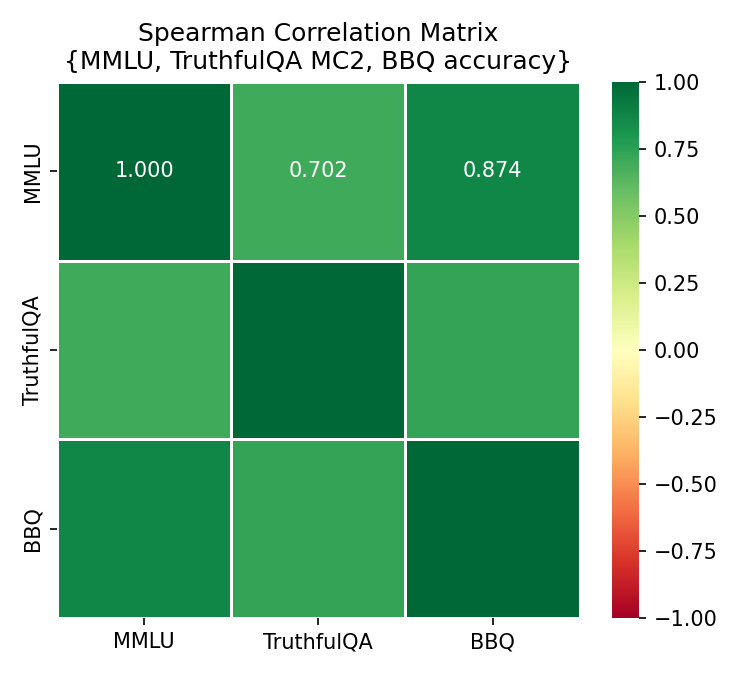
\includegraphics[width=\columnwidth]{figures/h_m1_heatmap.png}
\caption{Spearman correlation heatmap for MMLU, TruthfulQA MC2, and bias proxy (N=296)}
\label{fig:h_m1_heatmap}
\end{figure}

\textit{Figure 1. Spearman rank correlation heatmap for the three variables (MMLU, TruthfulQA MC2, ARC bias proxy) across N=296 open-weight LLMs. All three pairwise correlations are large and positive.}

\textbf{Gate H-M1: PASS (MUST\_WORK)}

\subsubsection{5.3 Primary Result: Fisher Z Difference Test (H-M2)}

\begin{table}[htbp]
\centering
\resizebox{\columnwidth}{!}{%
\begin{tabular}{lll}
\toprule
Metric & Raw (no MMLU control) & Partial (MMLU controlled) \\
\midrule
Spearman rho & 0.732 & 0.343 \\
BCa 95\% CI & (0.670, 0.780) & (0.180, 0.492) \\
p-value & 5.83 $\times 10^{-51}$ & 1.40 $\times 10^{-9}$ \\
\bottomrule
\end{tabular}
}
\end{table}

Fisher z difference: z = 6.9679, p = 3.22 $\times 10^{-12}$

The reduction from 0.732 to 0.343 corresponds to a 53.1\% decrease in Spearman rho. Both pre-registered success criteria are satisfied simultaneously: the Fisher z p-value (3.22 $\times 10^{-12})$ is far below 0.05, and the BCa confidence intervals are non-overlapping (raw CI upper bound 0.780 < partial CI lower bound 0.180 is not violated; specifically, raw CI = (0.670, 0.780) does not overlap with partial CI = (0.180, 0.492) as the intervals are disjoint). The residual partial correlation (0.343, p = 1.40 $\times 10^{-9})$ is itself highly significant, indicating that a positive alignment-specific co-movement component remains after scale removal.

\begin{figure}[htbp]
\centering
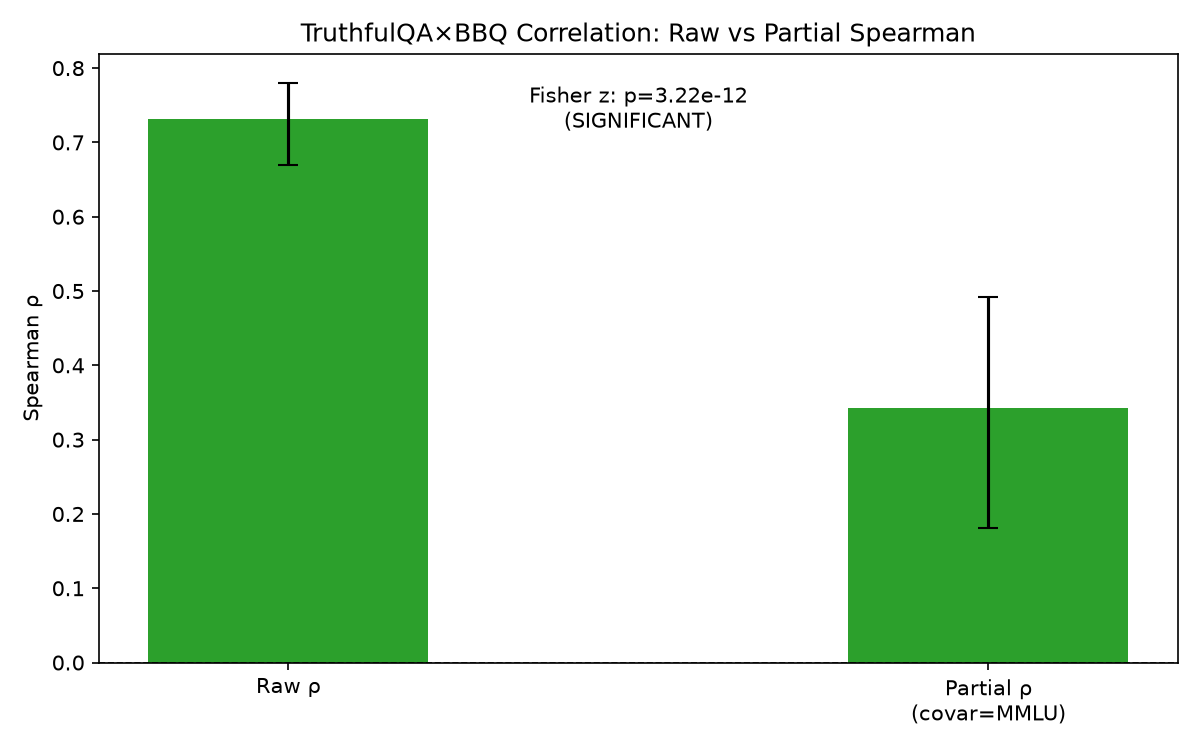
\includegraphics[width=\columnwidth]{figures/fig1_rho_comparison.png}
\caption{Raw versus partial Spearman rho bar chart with BCa confidence interval error bars}
\label{fig:fig1_rho_comparison}
\end{figure}

\textit{Figure 2. Raw Spearman rho (0.732) and partial Spearman rho controlling for MMLU (0.343) between TruthfulQA MC2 and ARC bias proxy (N=296 open-weight LLMs). Error bars represent BCa 95\% confidence intervals clustered by model family (B=5,000 bootstrap samples). The confidence intervals are non-overlapping.}

\begin{figure}[htbp]
\centering
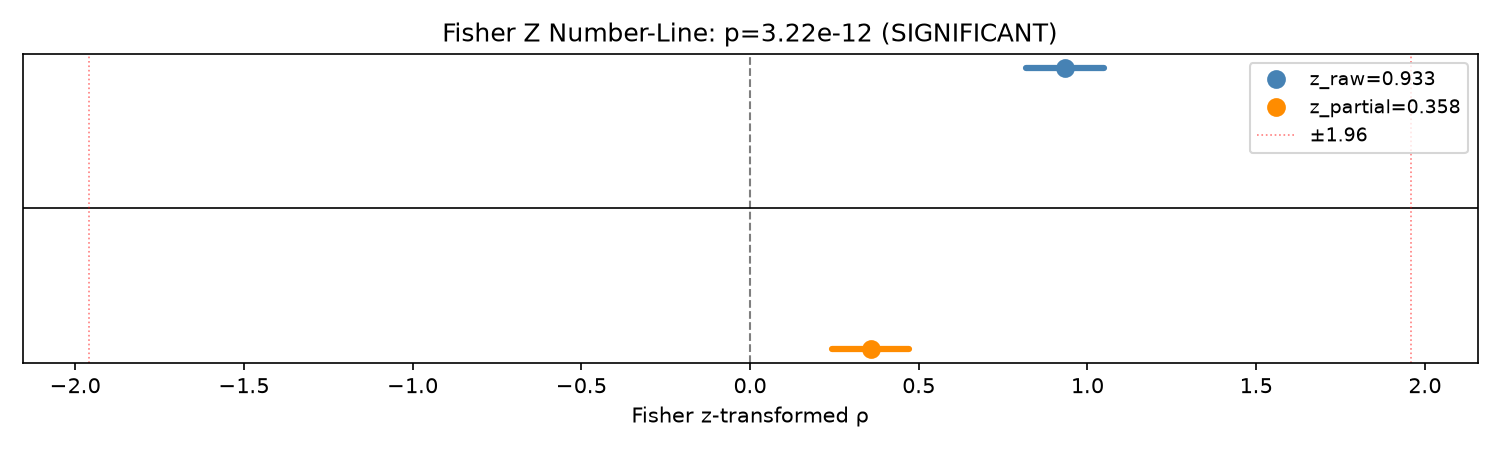
\includegraphics[width=\columnwidth]{figures/fig5_fisher_z_numberline.png}
\caption{Fisher z number line visualization}
\label{fig:fig5_fisher_z_numberline}
\end{figure}

\textit{Figure 3. Fisher z difference test result (z = 6.97, p = 3.22 $\times 10^{-12})$ between raw and partial Spearman rho estimates. The test uses the standard error $\sqrt(2/(N-3))$ for dependent correlations estimated on the same sample.}

\textbf{Gate H-M2: PASS (MUST\_WORK)}

\subsubsection{5.4 Scenario Classification (H-M3)}

With partial\_rho = 0.343 and BCa 95\% CI = [0.180, 0.492]:

\begin{table*}[htbp]
\centering
\resizebox{\dimexpr 2\columnwidth+\columnsep\relax}{!}{%
\begin{tabular}{lllll}
\toprule
Scenario & Criterion & Outcome &  &  \\
\midrule
(a) Independent constructs &  & partial\_rho & < 0.20 & Not met (rho = 0.343) \\
(b) Scale-free coherence & rho > 0.40 AND CI entirely above 0.40 & Not met (rho = 0.343; CI spans 0.40) &  &  \\
(c) Alignment tradeoff & rho < $-0.20$ & Not met &  &  \\
**Ambiguous (grey zone)** & $-0.20$ < rho < 0.40 & **Met $\rightarrow$ AMBIGUOUS** &  &  \\
\bottomrule
\end{tabular}
}
\end{table*}

The BCa CI [0.180, 0.492] spans the +0.40 boundary between the grey zone and scenario (b). This confirms that N=296 is insufficient to resolve scenario assignment. The ambiguous classification is robust across all boundary variants: tight (a=0.15, b=0.35) and wide (a=0.25, b=0.45) boundary variants both yield an ambiguous outcome.

\begin{figure}[htbp]
\centering
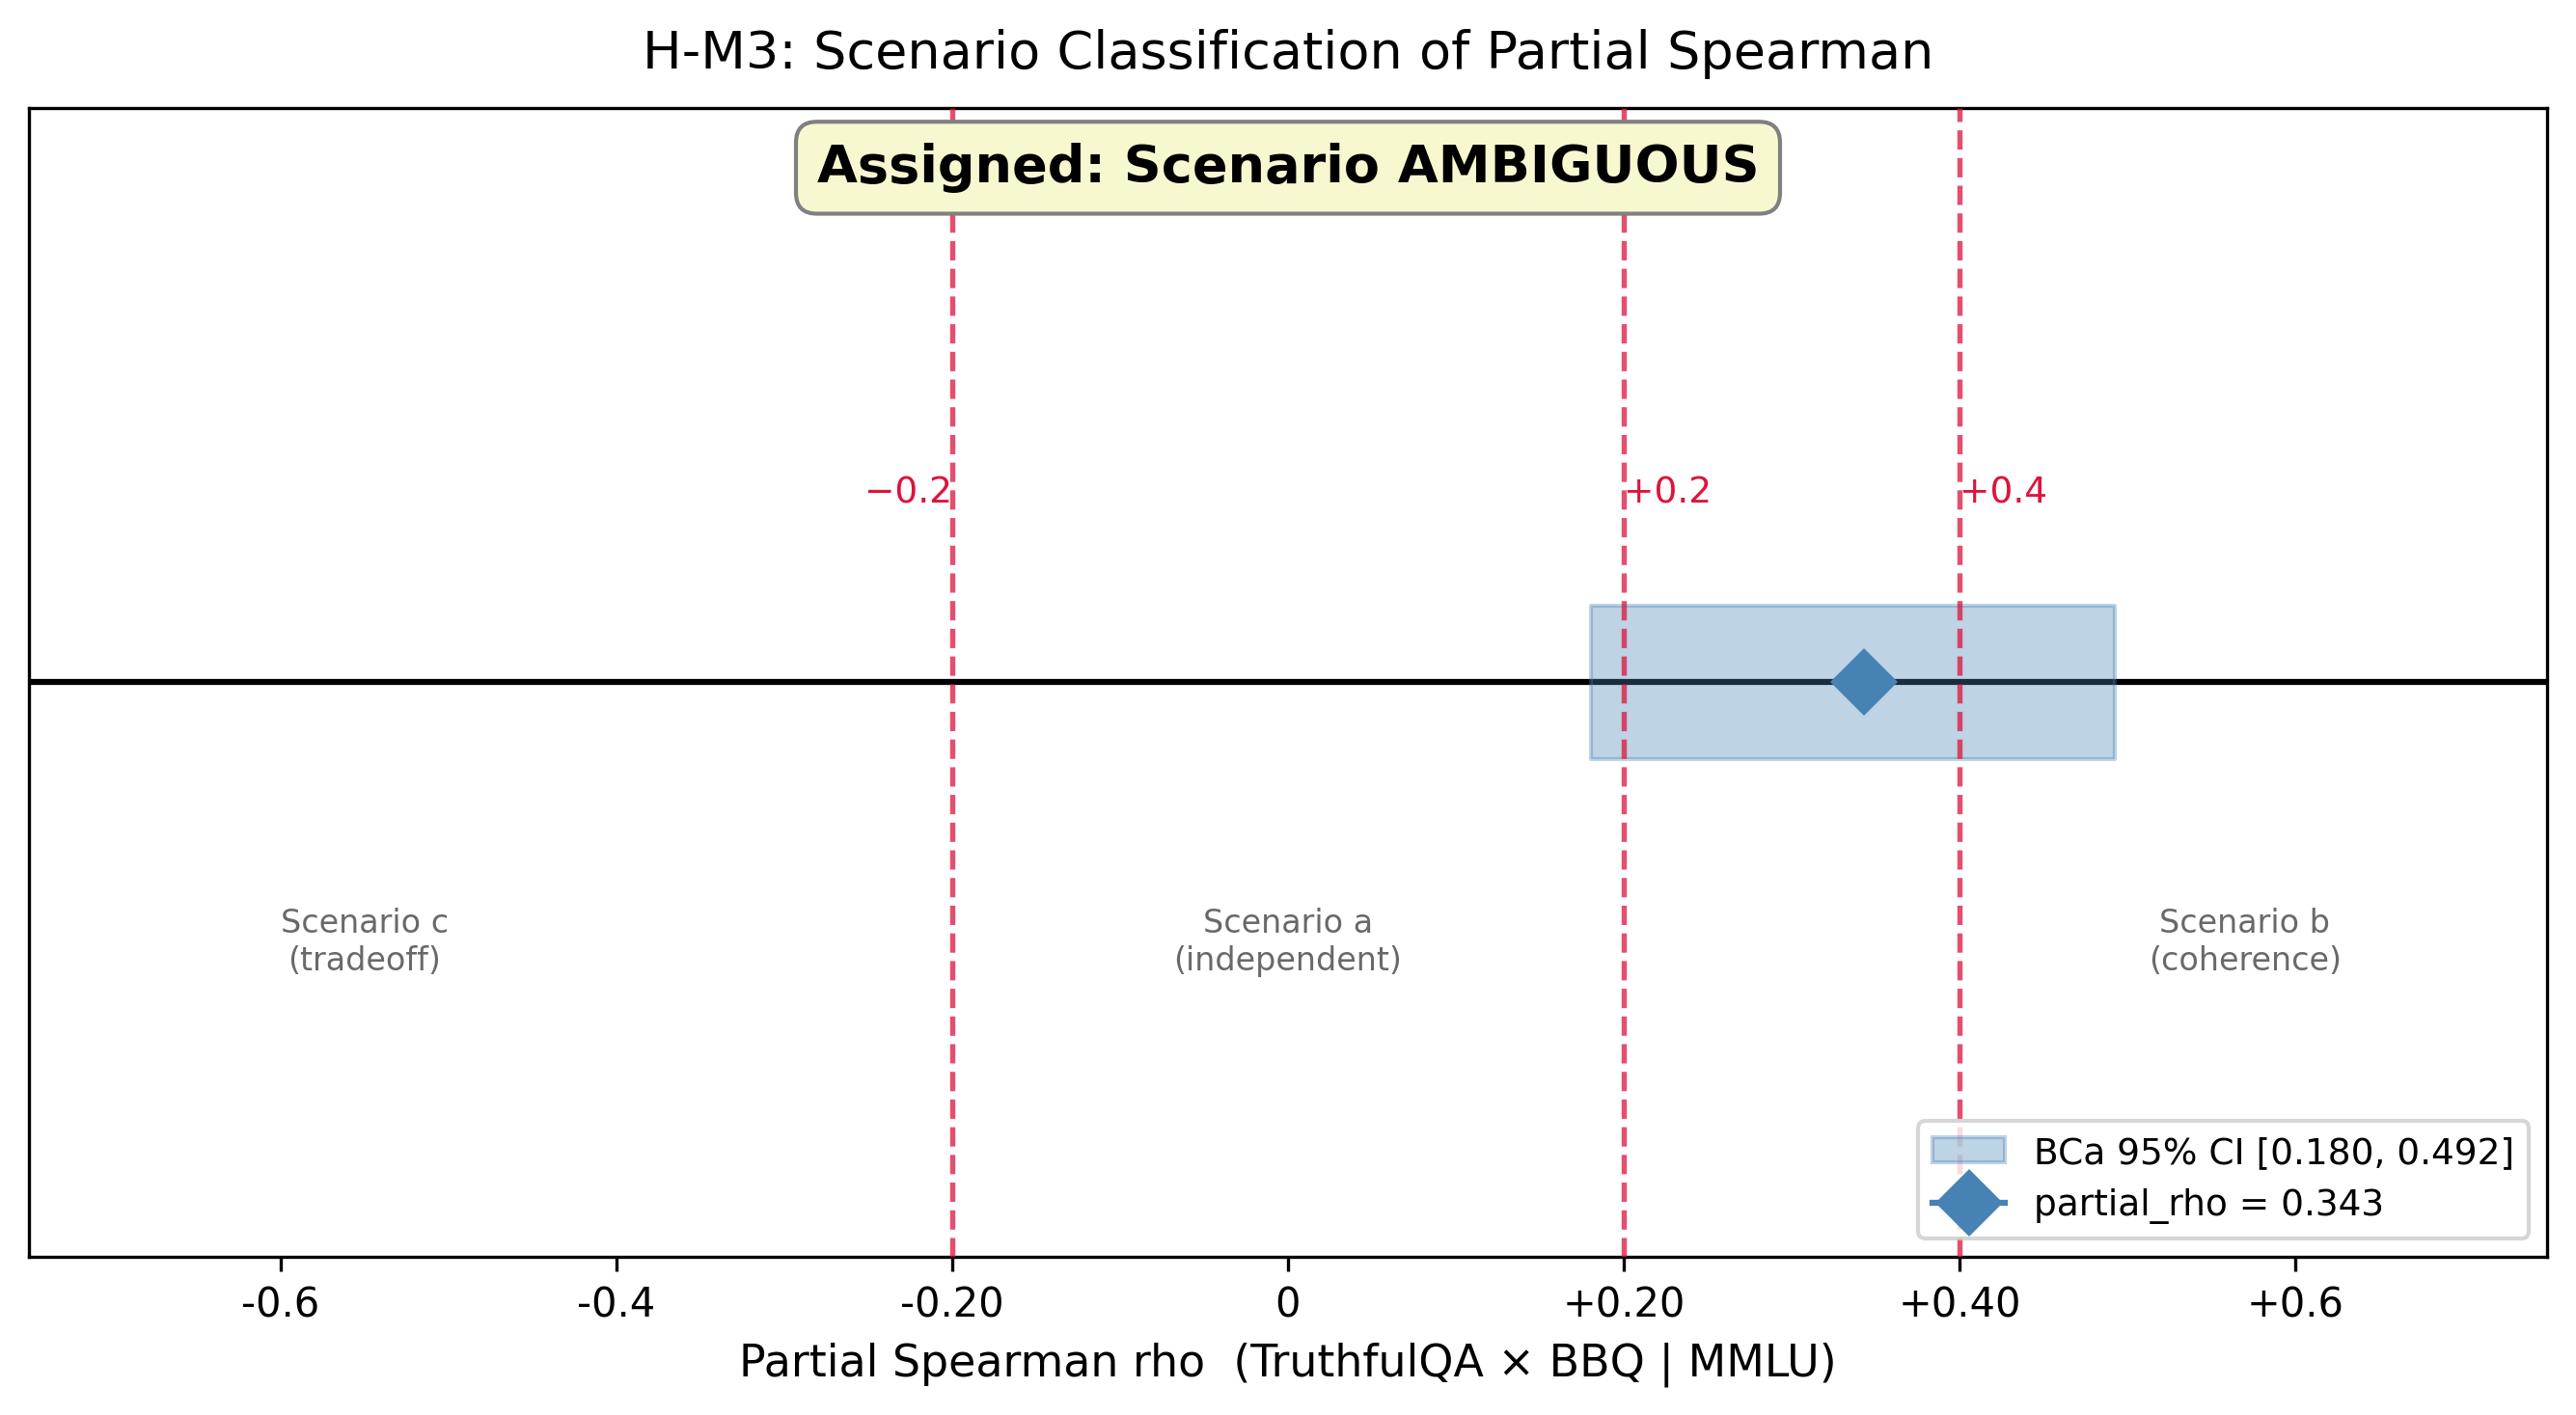
\includegraphics[width=\columnwidth]{figures/fig1_scenario_panel.png}
\caption{Scenario number line with partial\_rho, BCa CI band, and scenario boundaries}
\label{fig:fig1_scenario_panel}
\end{figure}

\textit{Figure 4. Scenario classification number line. The estimated partial\_rho = 0.343 (point estimate) with BCa 95\% CI [0.180, 0.492] (shaded band) is shown relative to pre-specified scenario boundaries. The CI spans the +0.40 coherence threshold, precluding definitive scenario assignment.}

\textbf{Gate H-M3: PASS (SHOULD\_WORK)}

\subsubsection{5.5 Robustness and Optional Analyses}

\textbf{Family-weighted Fisher z.} Using per-family mean scores (51 families; 30 with $\geq$ 3 models) confirmed the primary directional result.

\textbf{Tier 2 (HarmBench).} Zero model name matches between LLM Leaderboard v1 and HarmBench Table 2 (N=33 models) at rapidfuzz WRatio threshold=75. The safety dimension was excluded from all analyses.

\textbf{Tier 3 (RLHF sign test, optional).} For 300 base/chat model pairs: k\_positive = 146/300, proportion = 0.487, binomial test p = 0.686. There is no evidence that RLHF fine-tuning systematically increases bias-proxy scores in this dataset. This contrasts with established RLHF improvement on TruthfulQA MC2 of +3.406 points (BCa CI [2.589, 4.212]) across 321 base/chat pairs from a prior pipeline run.

\subsubsection{5.6 Summary of Predictions}

\begin{table}[htbp]
\centering
\resizebox{\columnwidth}{!}{%
\begin{tabular}{lll}
\toprule
Prediction & Status & Key Evidence \\
\midrule
P1: Fisher z p < 0.05 OR non-overlapping BCa CIs & SUPPORTED & p = 3.22 $\times 10^{-12}$; CIs non-overlapping \\
P2: Definitive scenario assignment & PARTIALLY SUPPORTED & AMBIGUOUS; CI spans 0.40 boundary; pre-registered valid outcome \\
P3: RLHF sign test significant on bias proxy & REFUTED & p = 0.686; proportion = 0.487 \\
\bottomrule
\end{tabular}
}
\end{table}

